%===================================================================
\section{Low Field Resonances}\label{sec:4b}
%===================================================================

\subsection{Experimental principle}
In a weak magnetic field the $F$-manifold splits linearly as
$E(F,m_F) = E_F + g_F \mu_B B\,m_F$, so transitions between adjacent
$m_F$ sublevels satisfy
\begin{equation}
  h\nu = g_F \mu_B B_{\mathrm{total}},
  \label{eq:zeeman}
\end{equation}
with $g_F \approx \pm 2/(2I+1)$ for the $^2S_{1/2}$ ground state (Eqs.~2B-8
and 2F-1 of Ref.~\cite{OpticalPumpingRubidium2002}). Circularly polarised
D$_1$ light pumps the atoms into the $|F,m_F=+F\rangle$ dark state,
rendering the cell transparent; a transverse RF field at the resonance
frequency Eq.~\ref{eq:zeeman} drives $\Delta m_F = \pm 1$ transitions out of
that dark state and restores absorption, producing a dip in the transmitted
intensity. The slope of $\nu$ versus the sweep-coil current therefore
calibrates the coil constants and, through the $g_F$ ratio of the two
isotopes, determines their nuclear spins. Deviations from
Eq.~\ref{eq:zeeman} at higher field are treated in Section~\ref{sec:4c}.

\subsection{Settings}
The optical axis was aligned with the horizontal component of the ambient
field, and circularly polarised D$_1$ light was passed through the cell as
described in Section~\ref{sec:common_procedure}. The sweep field was ramped
at ${\sim}\SI{1}{\hertz}$ so that the pumping dynamics reached a
quasi-steady state at each field value. Two measurement regimes were used:
(i)~for RF frequencies \SIrange{70}{200}{\kilo\hertz} the main-field coils
were disconnected and the field was supplied entirely by the sweep coils;
(ii)~for \SIrange{200}{1000}{\kilo\hertz} the main-field coils were
energised in the same direction as the sweep coils, with sweep fine-tuning.
Between five and six valid sweep cycles per RF frequency were aggregated
with combined Type~A and Type~B uncertainties.

\subsection{Zero-field resonance and Zeeman dips}
Figure~\ref{fig:4b_raw_traces} compares the photodetector signal during a
sweep with RF off (upper panel) and RF at \SI{150}{\kilo\hertz} (lower
panel). With no RF applied, a single absorption feature appears at the
sweep current that cancels the residual field: the Zeeman sublevels become
degenerate, optical pumping can no longer create a population imbalance
among $m_F$ states~\cite{OpticalPumpingRubidium2002}, and the atoms absorb
more D$_1$ light. With RF applied, two additional dips appear at higher
sweep current, corresponding to the two rubidium isotopes; the lower-field
dip belongs to the larger-$g_F$ isotope since a smaller field satisfies
Eq.~\ref{eq:zeeman} at the same $\nu$.

\begin{figure}[ht]
  \centering
  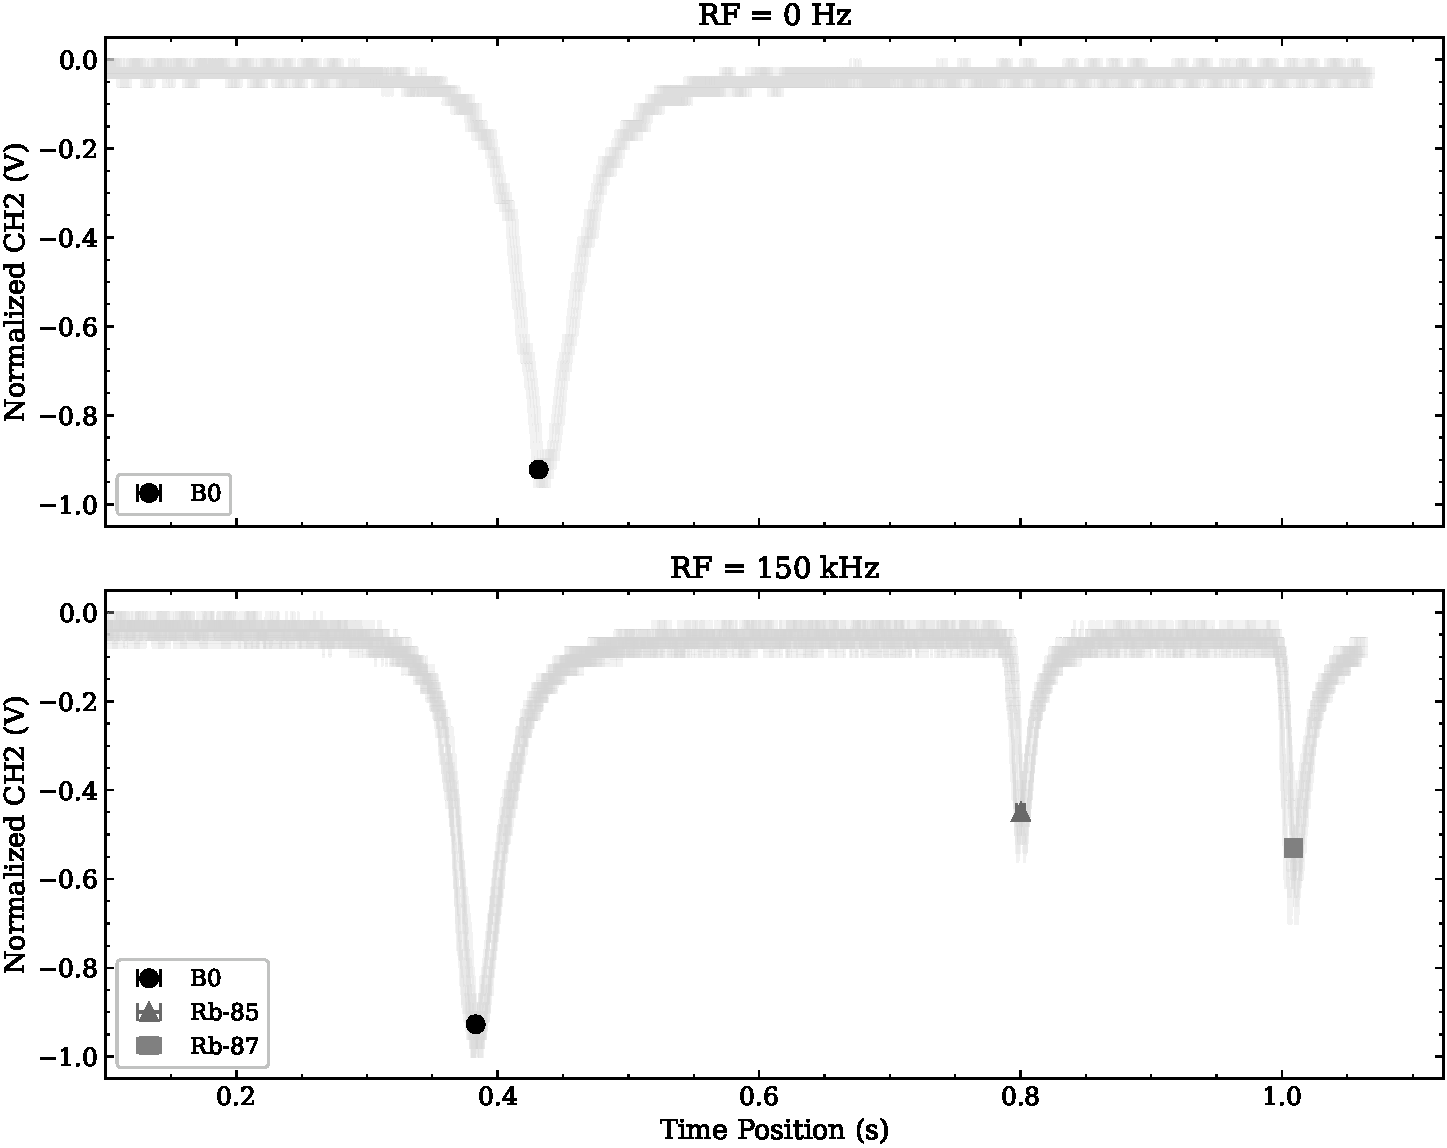
\includegraphics[width=0.7\linewidth]{figures/4b_raw_traces_comparison.pdf}
  \caption{Photodetector signal (CH2) during magnetic-field sweeps.
    \textbf{Upper:}~RF off, showing only the zero-field resonance (B0).
    \textbf{Lower:}~RF at \SI{150}{\kilo\hertz}, with the zero-field dip and
    the two Zeeman resonances (the lower-current one is $^{87}$Rb; see
    Section~\ref{sec:nuclear_spin}). Grey traces are individual sweep
    cycles; markers with horizontal error bars are the aggregated dip
    positions.}
  \label{fig:4b_raw_traces}
\end{figure}

\subsection{Low-field Zeeman effect and nuclear spin determination}\label{sec:nuclear_spin}
For each RF frequency in \SIrange{70}{200}{\kilo\hertz} the sweep-coil
current at each Zeeman resonance was recorded. Weighted linear fits of
$\nu(I_{\mathrm{sweep}})$ for the two isotopes (Fig.~\ref{fig:4b_low_field_zeeman})
yield
\begin{align}
  \text{steeper:}\quad \nu   & = 0.4634(56)\,I_{\mathrm{sweep}} - 0.1657(31)
  \quad [\mathrm{MHz},\,\mathrm{A}], \label{eq:fit_steep}                   \\
  \text{shallower:}\quad \nu & = 0.2981(23)\,I_{\mathrm{sweep}} - 0.1063(15)
  \quad [\mathrm{MHz},\,\mathrm{A}]. \label{eq:fit_shallow}
\end{align}
Since $\nu \propto g_F\,I_{\mathrm{sweep}}$, the slope ratio equals the
$g_F$ ratio: $m_1/m_2 = 0.4634/0.2981 = 1.554(22)$. In the low-field
Breit--Rabi limit~\cite{OPTOpticalPumping2024},
$\nu/B = 2.799/(2I+1)$ MHz/G, so the two-isotope ratio is
$(2I_2+1)/(2I_1+1)$. Equating this to $1.554$ with half-integer $I$ gives
$I_1 = 3/2$ and $I_2 = 5/2$ (ratio $6/4 = 1.500$): the steeper line is
$^{87}$Rb ($g_F = 1/2$) and the shallower line is $^{85}$Rb
($g_F = 1/3$), in agreement with the tabulated nuclear spins.\footnote{The
  automated dip-tagging pipeline assigns preliminary isotope labels from the
  sweep order; the correct identification is fixed here from the measured
  $g_F$ ratio.}

\begin{figure}[ht]
  \centering
  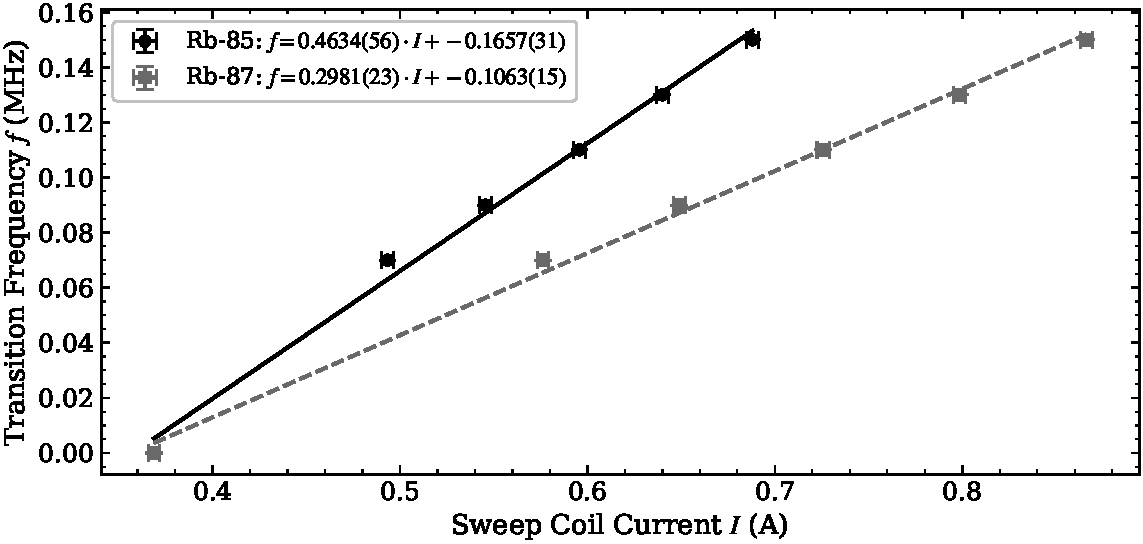
\includegraphics[width=0.7\linewidth]{figures/4b_low_field_zeeman.pdf}
  \caption{RF transition frequency vs.\ sweep-coil current for both
    isotopes. The steeper fit is $^{87}$Rb ($g_F=1/2$) and the shallower
    is $^{85}$Rb ($g_F=1/3$). Error bars are the combined Type~A$\oplus$B
    uncertainty in the sweep current.}
  \label{fig:4b_low_field_zeeman}
\end{figure}

\subsection{Sweep field calibration}\label{sec:sweep_cal}
Inverting Eq.~\ref{eq:zeeman} with the established $g_F$ values gives a
magnetic field at each data point, $B = h\nu/(g_F\mu_B)$. A single
weighted regression combining both isotopes and the $\nu=0$ reference
(Fig.~\ref{fig:4b_sweep_cal}) yields
\begin{equation}
  B = 0.6397(39)\,I_{\mathrm{sweep}} + (-0.2263(24))
  \quad [\mathrm{G},\,\mathrm{A}].
  \label{eq:sweep_cal}
\end{equation}
The slope $k_{\mathrm{sweep}} = 0.6397(39)\,\si{\gauss\per\ampere}$ is
the sweep-coil constant in Helmholtz configuration, and the intercept
$B_0 = -0.2263(24)\,\si{\gauss}$ is the residual field along the
optical axis (negative sign: residual opposes sweep direction). The
magnitude $|B_0| \approx \SI{0.23}{\gauss}$ is consistent with the
horizontal component of the geomagnetic field in Taipei
(${\sim}25^\circ$\,N, total \SIrange{0.35}{0.45}{\gauss}). As an
independent check, setting $\nu=0$ in
Eqs.~\ref{eq:fit_steep}--\ref{eq:fit_shallow} gives
$I_{\mathrm{sweep}}^{(0)} = 0.3575(80)\,\mathrm{A}$ and $0.3567(58)\,\mathrm{A}$,
confirming a common zero-field point across the two isotopes.

\begin{figure}[ht]
  \centering
  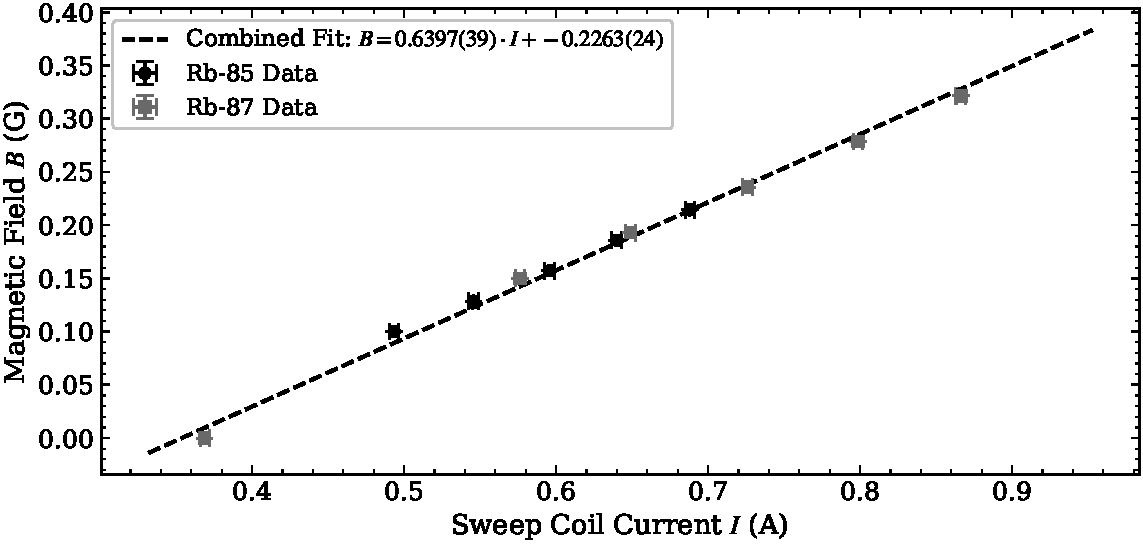
\includegraphics[width=0.7\linewidth]{figures/4b_sweep_field_calibration.pdf}
  \caption{Sweep field calibration. Magnetic field (computed from each
    resonance via $B=h\nu/(g_F\mu_B)$) plotted against sweep-coil current
    for both isotopes. Dashed line: combined weighted fit
    (Eq.~\ref{eq:sweep_cal}).}
  \label{fig:4b_sweep_cal}
\end{figure}

\subsection{Main field calibration}\label{sec:main_cal}
Above \SI{200}{\kilo\hertz} the sweep coils alone are insufficient and the
main coils were energised. At each operating point the total field was
obtained from $\nu$ and $g_F$, the sweep contribution (and residual) was
subtracted using Eq.~\ref{eq:sweep_cal} with full uncertainty propagation,
and the remainder was plotted against $I_{\mathrm{main}}$. A combined
weighted fit (Fig.~\ref{fig:4b_main_cal}) gives
\begin{equation}
  B_{\mathrm{main}} = 8.579(24)\,I_{\mathrm{main}} + 0.0059(22)
  \quad [\mathrm{G},\,\mathrm{A}].
  \label{eq:main_cal}
\end{equation}
The near-zero intercept ($0.0059(22)\,\si{\gauss}$) confirms that
Eq.~\ref{eq:sweep_cal} correctly accounts for the residual and sweep
contributions. The main-coil constant $k_{\mathrm{main}} = 8.579(24)\,\si{\gauss\per\ampere}$ is ${\sim}13\times$ larger than
$k_{\mathrm{sweep}}$, consistent with the higher turn count. These two
calibrations provide the magnetic-field reference for Sections~\ref{sec:4c}
and~\ref{sec:4d}.

\begin{figure}[ht]
  \centering
  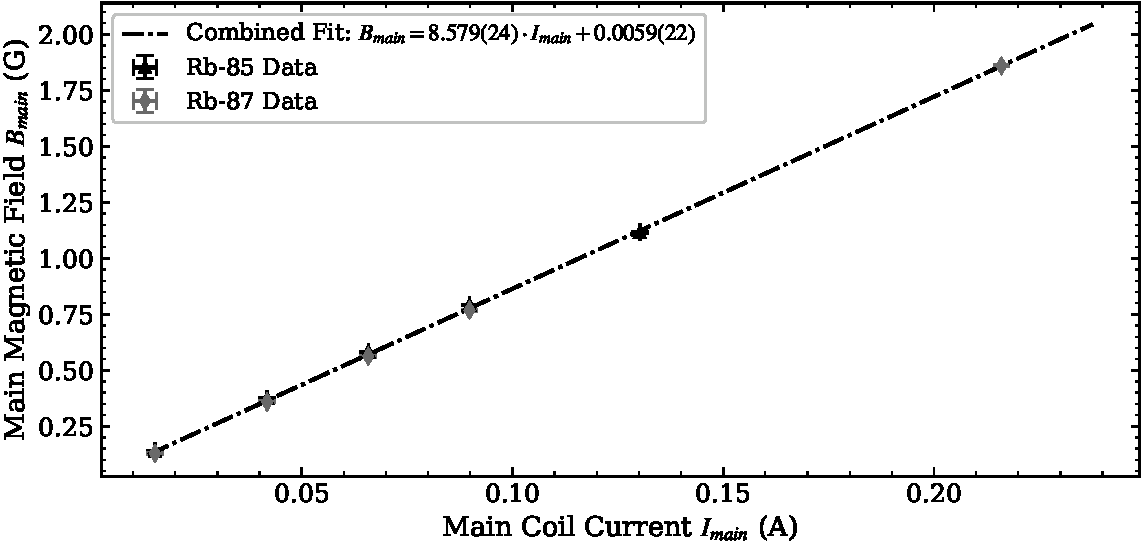
\includegraphics[width=0.7\linewidth]{figures/4b_main_field_calibration.pdf}
  \caption{Main field calibration. The field attributed to the main coils
    (total minus sweep and residual) plotted against main-coil current for
    both isotopes. Dash-dotted line: combined weighted fit
    (Eq.~\ref{eq:main_cal}).}
  \label{fig:4b_main_cal}
\end{figure}
